\documentclass[12pt]{article}

\usepackage{lipsum}
\usepackage{pgf-umlsd}
\usepackage[simplified]{pgf-umlcd}
\usepackage{float}
\usepackage{vhistory}
\usepackage{hyperref}
\usepackage{acro}
\usepackage{parskip}

\author{Tomislav Radanović, Rato Kuzmanić}
\title{Raccu Protocol Specification}
\date{\today}

\DeclareAcronym{sts}{
  short = STS,
  long  = secure token service,
  class = abbrev
}

\DeclareAcronym{ctap}{
  short = CTAP,
  long  = Client-to-Authenticator Protocol,
  class = abbrev
}

\begin{document}
    \begin{titlepage}
        \clearpage\maketitle
        \vfill
        \thispagestyle{empty}
    \end{titlepage}

    \clearpage\tableofcontents
    \thispagestyle{empty}
    \setcounter{page}{0}
    \newpage

    \section{Introduction}
This document provides a formal specification of the Raccu protocol. All readers are assumed to have a working 
knowledge in cryptography and computer networking. As this is a high-level overview, implementation details are 
omitted intentionally.

    \subsection{Background}
    Raccu is a centralized secure token service (STS) protocol for public-key cryptography authentication 
    based on a smartphone biometry. The protocol is architecturally inspired by the likes of OAuth 2.0, OpenID, 
    and W3C's WebAuthn while it conceptually resembles FIDO Alliance's Client-to-Authenticator Protocol (CTAP), 
    namely FIDO UAF standards.

    \subsection{Goals}
    The core vision of Raccu is to provide a user with a uniform method of authentication possessing the 
    following properties: 
        \begin{enumerate}
            \item Smaller complexity and lesser cognitive load than in a traditional email and password 
                  authentication system.
            \item Single registration process for authenticating to multiple web services and applications.
            \item Authentication process for issuing an attestation is independent of the type of registration 
                  used to create an account.
            \item Preserving data and origin integrity of the attestation through public key infrastructure (PKI) 
                  based chain of trust.
            \item Requiring user's consent via independent biometric authorization process before granting an 
                  attestation.
        \end{enumerate}

    \subsection{Disclaimer}
    Implementation of certain elements of this specification may require licenses under third party intellectual 
    property rights, including without limitation, patent rights. The authors and any other contributors to this 
    specification are not, and shall not be held, responsible in any manner for identifying or failing to identify 
    any or all such third party intellectual property rights.    
    
    \medskip
    THIS SPECIFICATION IS PROVIDED “AS IS” AND WITHOUT ANY WARRANTY OF ANY KIND, INCLUDING, WITHOUT LIMITATION,
    ANY EXPRESS OR IMPLIED WARRANTY OF NON-INFRINGEMENT, MERCHANTABILITY OR FITNESS FOR A PARTICULAR PURPOSE.

    \subsection{Contributing}
    Anyone can contribute to the protocol or to its specification. To learn more about contributing, please visit our 
    official repository on GitHub located at \href{https://www.github.com/Raccu/Documentation}{https://www.github.com/Raccu/Documentation}.
    \newpage

    \section{Definitions}
Throughout the specification a following list of terms is widely used. In this section their meaning and assumptions 
made on them are given in details.

\medskip
\textbf{Email}: Email client that allows the user to gain read access rights to the inbox associated
with the email address they provided. It is assumed that the user is the only person with this privilege.

\medskip
\textbf{Auth}: Central authentication provider that serves as a secure token store (STS) and conforms to 
the Raccu Auth Provider API Specification. Valid and trusted certificate issued by a certificate authority
(CA) as a part of PKI for this entity is implied.

\medskip
\textbf{Mobile}: An implementation of the mobile application that communicates with the corresponding Auth instance 
conforming to the Raccu Mobile Application Specification. Ability to authenticate the user via a fingerprint scanner
on the host smartphone is implied.

\medskip
\textbf{Browser}: An arbitrary web browser in charge of rendering quick response (QR) codes and dispatching appropriate 
messages as specified by the Raccu Client Component Specification.

\medskip
\textbf{Attestation}: Digitally signed claim in a form of a token that confirms holder's identity. Issued by 
Auth in a format defined in this specification.

\medskip
\textbf{Server}: An end web service or application that consumes an attestation. Authorization service within the 
Server is assumed. Valid and trusted certificate issued as a part of PKI for this entity is implied.

\medskip
The key words "MUST", "MUST NOT", "REQUIRED", "SHALL", "SHALL NOT", "SHOULD", "SHOULD NOT", "RECOMMENDED", 
"NOT RECOMMENDED", "MAY", and "OPTIONAL" in this document are to be interpreted as described in 
\href{https://tools.ietf.org/html/rfc2119}{RFC 2119} and \href{https://tools.ietf.org/html/rfc8174}{RFC 8174} 
when, and only when, they appear in all capitals, as shown here.

    \newpage

    \section{Register}

    \subsection{Register via email}
    The flow of registering an account via email (i.e. using an email verification claim) is shown in figure 1 and
    defined as follows:
    \begin{enumerate}
        \item A user MUST provide a valid name and a valid email.
        \item When Auth receives a valid registration request, email containing the verification code MUST 
                be dispatched to the provided email address.
        \item Upon receiving the verification code and entering it into the Mobile, the Mobile MUST provide 
                a method to generate, store, and retrieve public key and an interface for signing an arbitrary 
                message with the matching private key.
        \item Mobile MUST finish an account creation by submitting a name, email, generated public key, and 
                a digital signature of all of the previous parameters, with a REQUIRED addition of the 
                verification code, to the Auth.
    \end{enumerate}
  
    \begin{figure}[H]
    \centering
    \begin{sequencediagram}

        \newinst{A}{Email}{}
        \newinst[3]{B}{Mobile}{}
        \newinst[3]{C}{Auth}{}
        
        \tiny
        \begin{call}{B}{POST /verify/email {(email)}}{C}{200 OK {(token)}}\end{call}{B}
        \mess{C}{Send an email {(verification code)}}{A}
        \mess{A}{verification code}{B}
        \begin{call}{B}{POST /register/email {(token, email, PU\textsubscript{k}, Sign{(token\textbar\textbar email\textbar\textbar PU\textsubscript{k}\textbar\textbar verification code)})}}{C}{200 OK}\end{call}{B}

    \end{sequencediagram}
    \caption{Register via email protocol flow.}
    \label{fig:registerViaEmail}
\end{figure}

        \subsubsection{Requirements}
        The following requirements are made for a registration via email:
            \begin{enumerate}
                \item Provided email MUST NOT be associated with another account on Auth.\\
                \textit{Argument:} This is to prove that one user can only have a single account.

                \item Verification code MUST be at least 4 characters long and short lived, and MUST NOT be 
                    predictable.\\        
                \textit{Argument:} Verification code should posses a certain entropy and a level of randomness, 
                                just as well as a limited lifetime in order to reduce the likelihood of a 
                                successful brute-force attack.

                \item Verification code MUST NOT be revealed to third parties or sent over the network, except when
                    it's sent to the Email by Auth.\\        
                \textit{Argument:} Verification code represents a shared secret between the entities and revealing 
                                it to other parties or sending it over a (potentially insecure) network poses 
                                a confidentiality breach risk. 

                \item It is RECOMMENDED to reset verification code after a several unsuccessful verification 
                    code entries.\\        
                \textit{Argument:} This is to reduce a chance of a successful brute-force attack.

                \item Mobile MUST NOT expose private key directly.\\
                \textit{Argument:} Since the digital signature is a basis of authentication, an utmost respect to 
                                protecting the confidentiality of the private key should be implemented.

                \item Mobile MUST always require a biometric authentication to allow access to digital signing 
                    capability.\\        
                \textit{Argument:} This is to avoid phishing attacks or other illegal attempts to get the user's 
                                digital signature without his/hers explicit approval.

                \item Mobile MUST store generated keys in a trusted execution environment (TEE).\\        
                \textit{Argument:} This is to avoid a root attack or other system-level attacks that target storage 
                                memory or execution environment.

                \item The communication between a Mobile and Auth MUST rely on a secure channel that provides 
                    confidentiality and verifies integrity. It is RECOMMENDED to use up-to-date version of 
                    Transport Level Security (TLS) protocol with a well-tested and computationally secure 
                    cipher suite.\\      
                \textit{Argument:} Mobile and Auth exchange user's personal information and transmitting them over a 
                                public channel would pose a privacy concern, as well as create new vectors of attack, 
                                namely social engineering, phishing, and targeted brute-force attacks.
            \end{enumerate}
        
    \subsection{Successful registration}
    If the registration via email is successful, the Mobile MUST remember user's name, email, public key, and 
    have access to the procedure that signs an arbitrary message with the matching private key. The Auth MUST 
    remember user's name, email, and public key.

    \subsection{Unsuccessful registration}
    If the registration via email fails for any reason related to the semantics of the protocol, an attempt to
    register MUST be discarded and all of the related data should be deleted. It is RECOMMENDED to log an attempt
    in order to screen a source of multiple invalid requests. Any of the following reasons is considered to be
    a semantic of the protocol:
        \begin{itemize}
            \item Email is already associated with another account.
            \item Verification code entered into Mobile does not match an expected verification code.
            \item The signature cannot be verified with a given public key.
            \item The signature is invalid.
        \end{itemize}
    If the registration fails for any other reason (e.g. network outage), an appropriate message SHOULD be
    dispatched or left to the other protocols for handling, should they offer such capability.

    \newpage

    \section{Login}
    \lipsum[1]
    \subsection{Sequenced diagram}
    \begin{figure}[H]
        \centering
        \begin{sequencediagram}
            
            \newinst{A}{Mobile}{}
            \newinst[2]{B}{Web}{}
            \newinst[2]{C}{Auth}{}
            \newinst[2]{D}{Server}{}

            \tiny
            \begin{call}{B}{GET /resource/limited/1}{D}{401 Unauthorized}\end{call}{C}
            \begin{call}{B}{GET /auth}{C}{200 OK {(challenge)}}\end{call}{B}
            \mess{B}{QR{(challenge, domain)}}{A}
            \begin{call}{A}{POST /token {(challenge, email, domain, Sign{(...)})}}{C}{200 OK}\end{call}{A}
            \mess{C}{Confirmation successful}{B}
            \begin{call}{B}{GET /token/\{challenge\}}{C}{200 OK {(token)}}\end{call}{B}
            \begin{call}{B}{POST /login {(token)}}{D}{200 OK {(JWT, session cookie, ...)}}\end{call}{B}

        \end{sequencediagram}
        \caption{Login protocol flow}
    \end{figure}
    \subsection{Token}
    \lipsum[1]

    \begin{figure}[H]
        \centering
        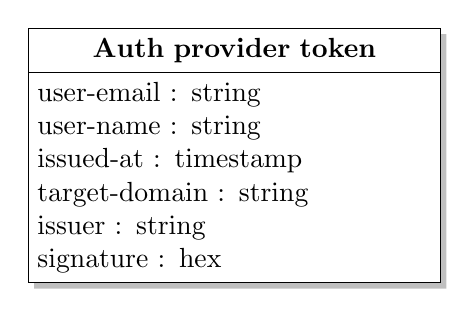
\begin{tikzpicture}
            \begin{class}[fill=white, drop shadow, draw=black]{Auth provider token}{0 ,0}
                \attribute{user-email : string}
                \attribute{user-name : string}
                \attribute{issued-at : timestamp}
                \attribute{target-domain : string}
                \attribute{issuer : string}
                \attribute{signature : hex}
            \end{class}
        \end{tikzpicture}
        \caption{Fields included into authentication token}
    \end{figure}

    \newpage

    \section{Reset credentials}
    \lipsum[1]
    \subsection{Sequenced diagram}
    \begin{figure}[H]
        \centering
        \begin{sequencediagram}

            \newinst{A}{Email}{}
            \newinst[3]{B}{Mobile}{}
            \newinst[3]{C}{Auth}{}

            \tiny
            \begin{call}{B}{POST /reset {(email)}}{C}{200 OK}\end{call}{B}
            \mess{C}{Email{(code)}}{A}
            \mess{A}{code}{B}
            \begin{call}{B}{POST /reset/verify {(email, code)}}{C}{200 OK {(reset token)}}\end{call}{B}
            \begin{call}{B}{POST /reset/\{reset token\} {(reset token, PUk, Sign(...))}}{C}{200 OK}\end{call}{B}

        \end{sequencediagram}
        \caption{Reset credentials protocol flow}
    \end{figure}
    \newpage

    \section{Delete account}
    \lipsum[1]
    \subsection{Sequenced diagram}
    \begin{figure}[H]
        \centering
        \begin{sequencediagram}

            \newinst{A}{Mobile}{}
            \newinst[5]{C}{Auth}{}

            \tiny
            \begin{call}{A}{DELETE / {(email, Sign{(...)})}}{C}{200 OK}\end{call}{A}
            
        \end{sequencediagram}
        \caption{Delete account protocol flow}
    \end{figure}
    \newpage

    \listoffigures\bigskip
    \printacronyms[include-classes=abbrev,name=Abbreviations]
    \begin{versionhistory}
        \vhEntry{0.0.0}{13.10.2018.}{Radanović}{Created document structure}
        \vhEntry{0.1.0}{18.10.2018.}{Radanović}{Added sequenced diagrams}
        \vhEntry{0.1.1}{23.10.2018.}{Radanović}{Updated sequenced diagrams}
        \vhEntry{0.2.0}{24.10.2018.}{Kuzmanić}{Added about project}
        \vhEntry{0.3.0}{25.10.2018.}{Kuzmanić}{Added introduction and definitions}
        \vhEntry{0.4.0}{25.10.2018.}{Kuzmanić}{Added registration via email}
    \end{versionhistory}
    
\end{document}
